%%%%%% Configurando os pacotes e comandos %%%%%%
%%%%%% Pule para a linha 62 %%%%%%%
\documentclass[fontsize=11pt]{article}
\usepackage[margin=0.70in]{geometry}
\usepackage{lipsum,mwe,abstract}
\usepackage[T1]{fontenc} 
\usepackage[brazilian]{babel} 
\usepackage{setspace}
\usepackage{caption}
\usepackage[hidelinks]{hyperref}
\usepackage{multirow}

\usepackage{fancyhdr} % Custom headers and footers
%\pagestyle{fancyplain} % Makes all pages in the document conform to the custom headers and footers
%\fancyhead{} 
%\fancyfoot[C]{\thepage} % Page numbering for right footer
\setlength\parindent{0pt} 
\setstretch{1.5}

\usepackage{amsmath,amsfonts,amsthm, amssymb} % Math packages
\usepackage{wrapfig}
\usepackage{graphicx}
\usepackage{float}
\usepackage{subcaption}
\usepackage{comment}
\usepackage{enumitem}
\usepackage{cuted}
\usepackage{sectsty} % Allows customizing section commands
% \allsectionsfont{\normalfont \large \scshape} % Section names in small caps and normal fonts
\usepackage{biblatex}
\addbibresource{references.bib}

%code things
\usepackage{xcolor}
\usepackage{listings}

\lstdefinestyle{customc}{
  belowcaptionskip=1\baselineskip,
  breaklines=true,
  frame=L,
  xleftmargin=\parindent,
  language=C,
  showstringspaces=false,
  basicstyle=\small\ttfamily,
  keywordstyle=\bfseries\color{green!40!black},
  commentstyle=\itshape\color{purple!40!black},
  identifierstyle=\color{blue},
  stringstyle=\color{orange},
}
%%%

\definecolor{codegreen}{rgb}{0,0.6,0}
\definecolor{codegray}{rgb}{0.5,0.5,0.5}
\definecolor{codepurple}{rgb}{0.58,0,0.82}
\definecolor{backcolour}{rgb}{0.95,0.95,0.92}

\lstdefinestyle{mystyle}{
  backgroundcolor=\color{white},   
  commentstyle=\color{codegreen},
  keywordstyle=\color{magenta},
  numberstyle=\tiny\color{codegray},
  stringstyle=\color{codepurple},
  basicstyle=\linespread{0.9}\ttfamily\footnotesize,
  breakatwhitespace=false,         
  breaklines=true,                 
  captionpos=b,                    
  keepspaces=true,                 
  numbers=left,                    
  numbersep=5pt,                  
  showspaces=false,                
  showstringspaces=false,
  showtabs=false,                  
  tabsize=2,
  language=C
}
\lstset{escapechar=@,style=mystyle}
  
  
  \renewenvironment{abstract} % Change how the abstract look to remove margins
  {\small
  \begin{center}
  \bfseries \abstractname\vspace{-.5em}\vspace{0pt}
  \end{center}
  \list{}{%
    \setlength{\leftmargin}{0mm}
    \setlength{\rightmargin}{\leftmargin}%
  }
  \item\relax}
 {\endlist}
 
\makeatletter
\renewcommand{\maketitle}{\bgroup\setlength{\parindent}{0pt}% Change how the title looks like
\begin{center}
    \textbf{
      Universidade de São Paulo\\
      Instituto de Ciências Matemáticas e Computação
    }
\end{center}
\begin{flushleft}
  \textbf{\@title}
  \@author\\
  [3pt] 
  \@date
\end{flushleft}\egroup
}
\makeatother
%%% Daqui pra cima é apenas configuração %%%
%%%%%%%%%%%%%%%%%%%%%%%%%%%%%%%%%%%%%%%%%%%%

%%%%%% Definindo seus dados %%%%%%
\title{
\Large{Relatório 3 de Laboratório de Introdução à Ciências da Computação 2}\\
[10pt] 
}
\author{Vítor Amorim Fróis} 
\date{\today}
%%%%%%%%%%%%%%%%%%%%%%%%%%%%%%%%%%%

%%%%%% Iniciando seu relatório %%%%%% 
\begin{document}
\maketitle

\begin{abstract}
    %%%%%% Contextualize o seu trabalho. %%%%%%%
    Durante o último módulo da matéria de Laboratório de ICC2, foram estudados métodos
    de ordenação que não utilizam comparação: Counting, Bucket e Radix, obtendo assim resultados melhores em diversas 
    situações. Apesar disso, existem limitações para esses algoritmos, que nem sempre funcionam tão bem.
    \\ Esse relatório busca analisar isso de modo a detalhar quando cada método pode ou não ser útil,
    além de comparar o que foi estudado ao longo do semestre.
\end{abstract}

\rule{\linewidth}{0.2pt}

\section{Introdução}
    %%%%%% Faça a introdução do seu relatório. O que será feito? %%%%%%
    Ao longo do último semestre, foram estudados diversos métodos de ordenação,
    alguns com complexidade melhor ou pior de acordo com as regras da 
    notação assintótica. \\
    É fato que dependendo da situação, cada algoritmo
    pode performar melhor ou pior. Até agora, entretanto, nenhum dos métodos
    estudados ultrapassa a barreira de $\Theta (n) = n \log n$. Entretanto, ao
    olhar o problema por outra forma é possível melhorar os métodos.
    Esse relatório possui como objetivo analisar tais métodos, trazendo suas análises 
    assintóticas, os melhores e piores casos, além de gráficos comparativos com o que 
    foi estudado nos últimos relatórios.

\section{Metodologia e desenvolvimento}
    \subsection{A barreira logarítmica}
        %%%%%% Explique a metodologia utilizada e o desenvolvimento do projeto. Como você obteve seus dados? Coloque seus códigos e embasamentos teóricos aqui se necessário. %%%%%%
        Ao longo dos últimos módulos foram estudados métodos que se utilizavam de comparações
        para ordenar. Tais algoritmos possuem um limite inferior que pode ser demonstrado a 
        partir de uma árvore de decisões binária. \Cite{mitclass} 
        \\Existem $n!$ resultados possíveis para um algoritmo de ordenação, isto é, a permutação de
        todos os elementos do vetor. Uma árvore de decisão do modelo que usa somente comparações
        deve possuir $n!$ folhas, e portanto uma altura de no mínimo 
        $\Omega(log(n!))$. É possível aplicar a aproximação de Stirling para encontrar
        que $n! = \sqrt{2 \pi n}(\dfrac{n}{e})^e$ ou considerar que $n!>(n/2)^{n/2}$. Assim:
        $$\log(n!) = \log(n/2)^{n/2}$$
        $$\log(n!) = \dfrac{n}{2}\log(n/2)$$
        $$\log(n!) = n\log(n)$$
        Isso nos leva a uma complexidade mínima de $\Theta(n)=n\log(n)$ \cite{mitvideo}.
        Entretanto, ao quebrar a barreira das comparações, é possível melhorar os algoritmos. 
        \subsection{Counting Sort}
        Como o próprio nome acusa, o Counting Sort é um algoritmo que se vale da contagem 
        a fim de ordenar sequências de números. Para isso, é necessário um vetor
        auxiliar de tamanho $k = \max - \min$, que incrementa o valor de das chaves
        de acordo com os índices do original. Logo, é necessário $O(n)$ para inserir 
        no vetor auxiliar e $O(k)$ ordenar no final.
        $$\text{Complexidade de tempo: } O(n+k)$$
        $$\text{Complexidade de memória: } O(k)$$
        Espera-se que o Counting Sort performe bem com números inteiros e chaves em
        pequenos intervalos, dado que para um $k$ muito grande, a complexidade do 
        algoritmo cresce muito. Diferente dos métodos estudados nos módulos 1 e 2, 
        a taxa de desordem do vetor não importa.
        \\Para o código a seguir e dos próximos métodos, considere que 
        $a$ representa operações aritméticas, $b$ atribuições, e $c$ comparações.
        \lstinputlisting[linerange={10-50}]{countingsort.c}
        \subsection{Bucket Sort}
        Ainda que a implementação do Counting Sort simples seja instável e seja 
        possível resolver isso através do uso de registros, outro método existe para
        solucionar tal problema. Através do uso de "baldes", o Bucket Sort realiza
        ordenação por contagem abaixo do limite anteriormente conhecido.
        \\De forma similar ao Counting, é necessário alocar um vetor de listas 
        ligadas de tamanho $k= \max - \min$, que representarão os baldes. 
        Cada balde pode armazenar um valor ou intervalo.
        \footnote[1]{Ao receber um intervalo, é possível, de acordo com a aplicação, 
        aplicar outro método de ordenação que funcione bem com pequenos vetores ou 
        intervalos para ordenar cada Bucket.}
        Com complexidade $O(n)$ os elementos são inseridos no vetor. Então, basta 
        esvaziar os baldes, ordenados, a partir da cabeça, inserindo no vetor 
        original $(k+n)$. 
        $$\text{Totalizando: } n+k+n+k \rightarrow 2(n+k)$$
        $$O(n+k) \text{ em tempo}$$
        Em termos de memória gasta, porém, devido ao uso de ponteiros nas listas ligadas, 
        existe uma constante $\epsilon$ \Cite{moacir}, tal que a complexidade de espaço é 
        $$O(n+k+\epsilon)$$ 
        Isso significa que o algoritmo possui complexidade muito semelhante 
        ao Counting Sort, porém usando mais memória auxiliar com o objetivo de 
        manter a estabilidade.
        \lstinputlisting[linerange={14-71}]{bucketsort.c}
    \subsection{Radix Sort}
        Essencialmente, os algoritmos vistos até agora são muito bons, mas ainda é possível fazer melhor.
        Para um $k$ muito grande, Counting e Bucket não são suficientes. Um método de ordenação
        mais enxuto é o Radix Sort. A ideia do algoritmo é dividir cada número em potências da 
        base utilizada e ordenar do menos significativo para o mais significativo com ajuda 
        de algum dos dois métodos anteriores para alcançar complexidade de tempo linear.
        \\ \textbf{Utilizando Counting Sort:} 
        Para um número qualquer na base $b$, o número de dígitos máximo $d$ pode ser representado 
        por $\log_bc+1$ e a complexidade será $d\times \text{Counting Sort}$. Como todos
        os algarismos estarão entre $0$ e $b$, a complexidade do counting será $O(n+b)$. 
        $$O((n+b)\times d) \text{ ou }$$ $$O((n+b)\times (\log_bc+1))$$
        Aqui, é importante encontrar uma boa base para diminuir a complexidade de tempo
        do algoritmo. Ao resolver, encontra-se $b=n$. \label{radix}
        $$O((n+n)\times (\log_nc+1)) \rightarrow O(n \log_nc)$$ Se $c \eqslantless n^{p}$, o algoritmo 
        se torna $O(np)$. \cite{mitvideo}
        Para o Radix funcionar, é necessário fazer algumas modificações no algoritmo de subrotina.
        \lstinputlisting[linerange={10-40}]{radix.c}
        Então, simples chamadas do método ordenam um vetor. 
        \lstinputlisting[linerange={41-53}]{radix.c}
        Veja que a complexidade ainda é logarítmica. Espera-se que com a escolha 
        correta de base, o algoritmo se torne linear. 

\section{Resultados}
    %%%%%% Mostre os resultados obtidos através dos cálculos. Utilize imagens se necessário. %%%%%%
    Para a seção de resultados, é importante repetir as mesmas experiências que foram realizadas com
    outros métodos afim de fazer boas comparações. Portanto, houveram testes de ordenação com vetores 
    de 5000 a 100000 elementos. Todos os vetores utilizados foram aleatórios, pois a falta de comparação
    nos algoritmos faz com que ordenação prévia não seja um fator importante na análise. 
    \\ Entretanto, como destacado na parte de Metodologia, a complexidade de tempo depende do 
    tamanho máximo do vetor $k$. Assim, para comparação desses 3 métodos, haverão 3 gráficos inicialmente,
    gerados a partir de vetores uniforme, denso e esparso. 
    \newpage
    \subsection{Vetor Uniforme}
      No vetor uniforme, os elementos são distribuídos de maneira uniforme pelo vetor. Ou seja, $k = n$, 
      e consequentemente, $O(n+k) \rightarrow O(2n)$  \label{uniforme}.
      É esperado que todos vetores sejam lineares, incluindo o Radix Sort que conta
      com a escolha adequada de $n$, descrita anteriormente, para alcançar complexidade $O(n)$.
      \begin{figure}[H]
        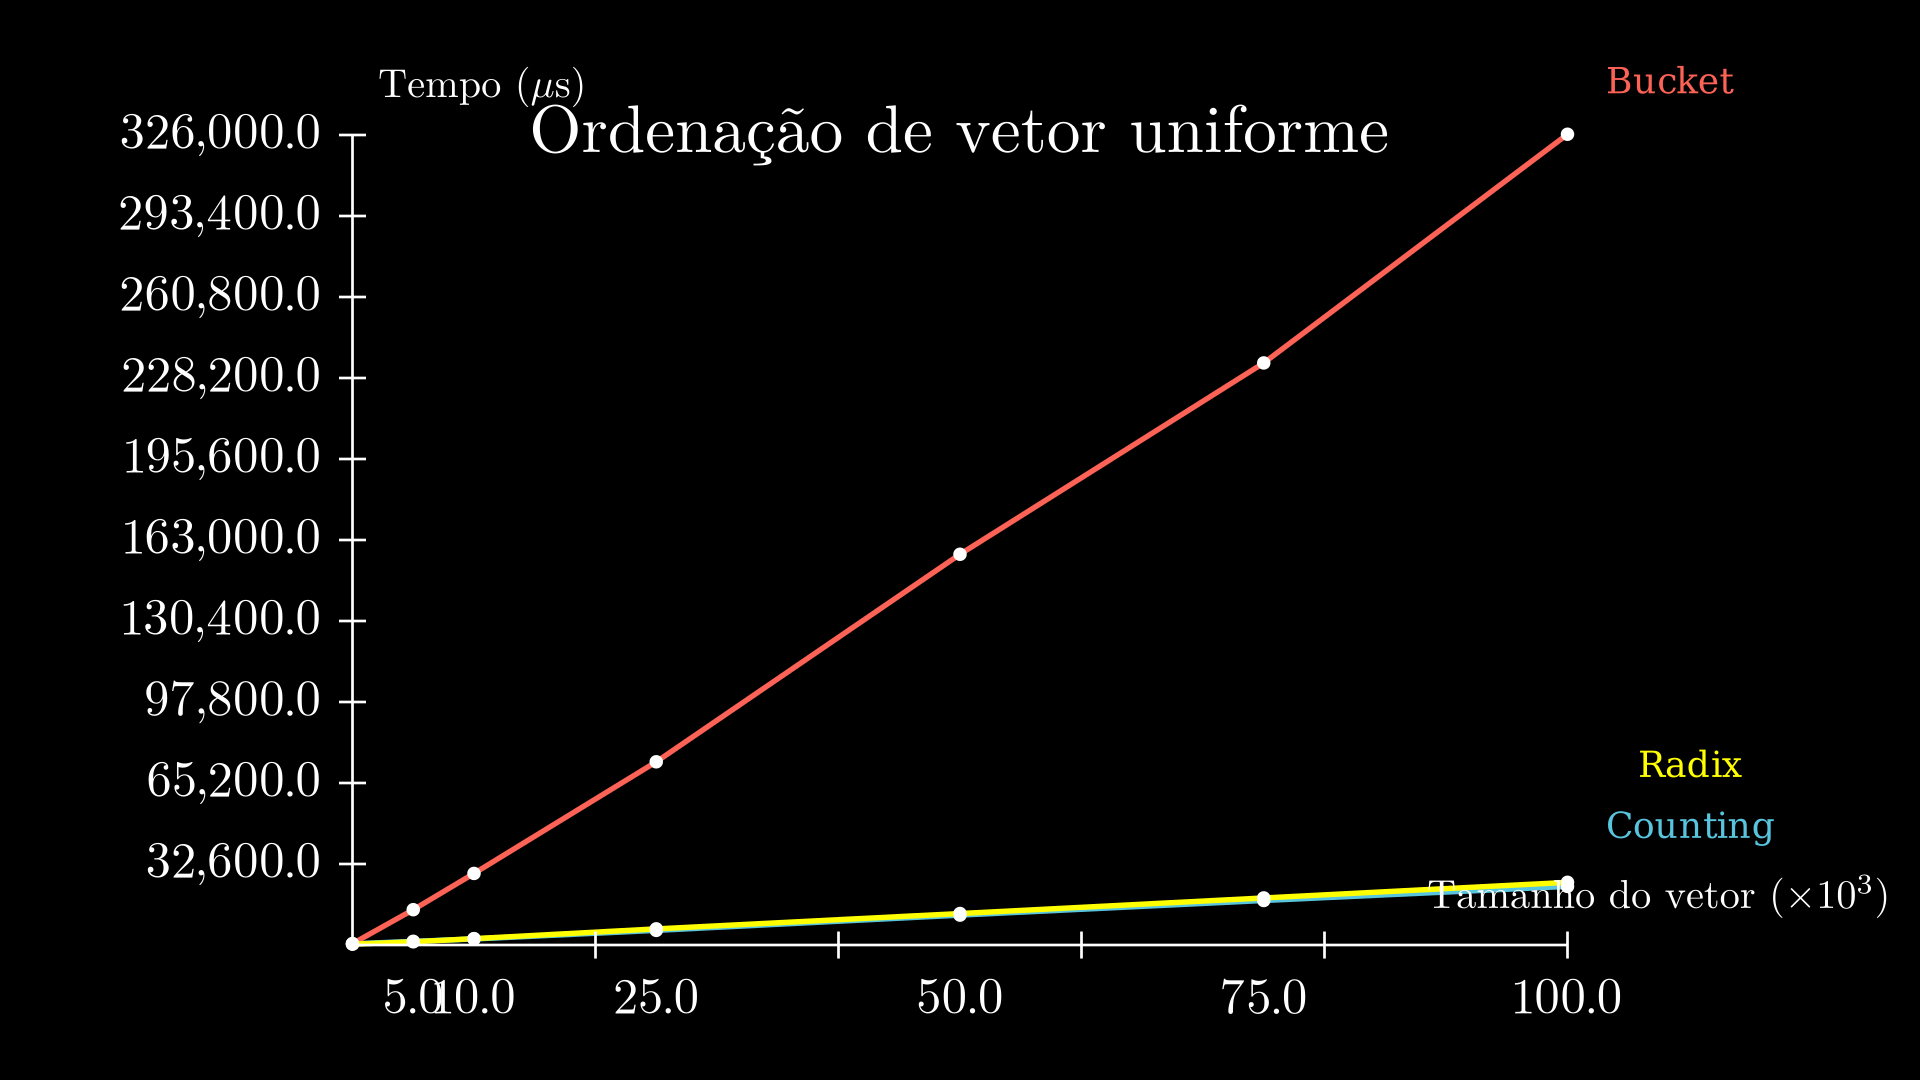
\includegraphics[width=\textwidth]{uniforme.png} 
        \caption{Ordenação de vetores uniformes com até 100000 elementos}
        \label{fig:uniforme}
      \end{figure}
      De fato, os vetores cumprem a linearidade, contudo, o Bucket Sort performa muito pior que os outros.
      Isso acontece devido as constantes excluídas na análise assintótica, fator que interferiu 
      em análises passadas também. 
      Além disso, é possível perceber que Counting e Radix ficam bem próximos. E isso se deve ao fato de
      que para vetores uniformes, o Radix é apenas um Counting Sort.
      \newpage
    \subsection{Vetor Denso}
      Já no vetor denso, os elementos possuem tamanho máximo de $\dfrac{1}{100}$ do número de elementos. Isso
      significa que há diversas repetições, cenário em que os algoritmos analisados melhor devem atuar, 
      pois considerando que a complexidade média é $O(n+k)$ e quando $k=\dfrac{n}{100}$, 
      $$O(n+\dfrac{n}{100}) < O(n+n) \text{. Veja } \ref{uniforme}$$ 
      $$\text{A fração é desprezível: }O(n) < O(2n).$$
      Assim, os métodos devem apresentar desempenho 2 vezes mais rápido que no vetor uniforme. 
      \begin{figure}[H]
        \caption{Ordenação de vetores densos com até 100000 elementos}
        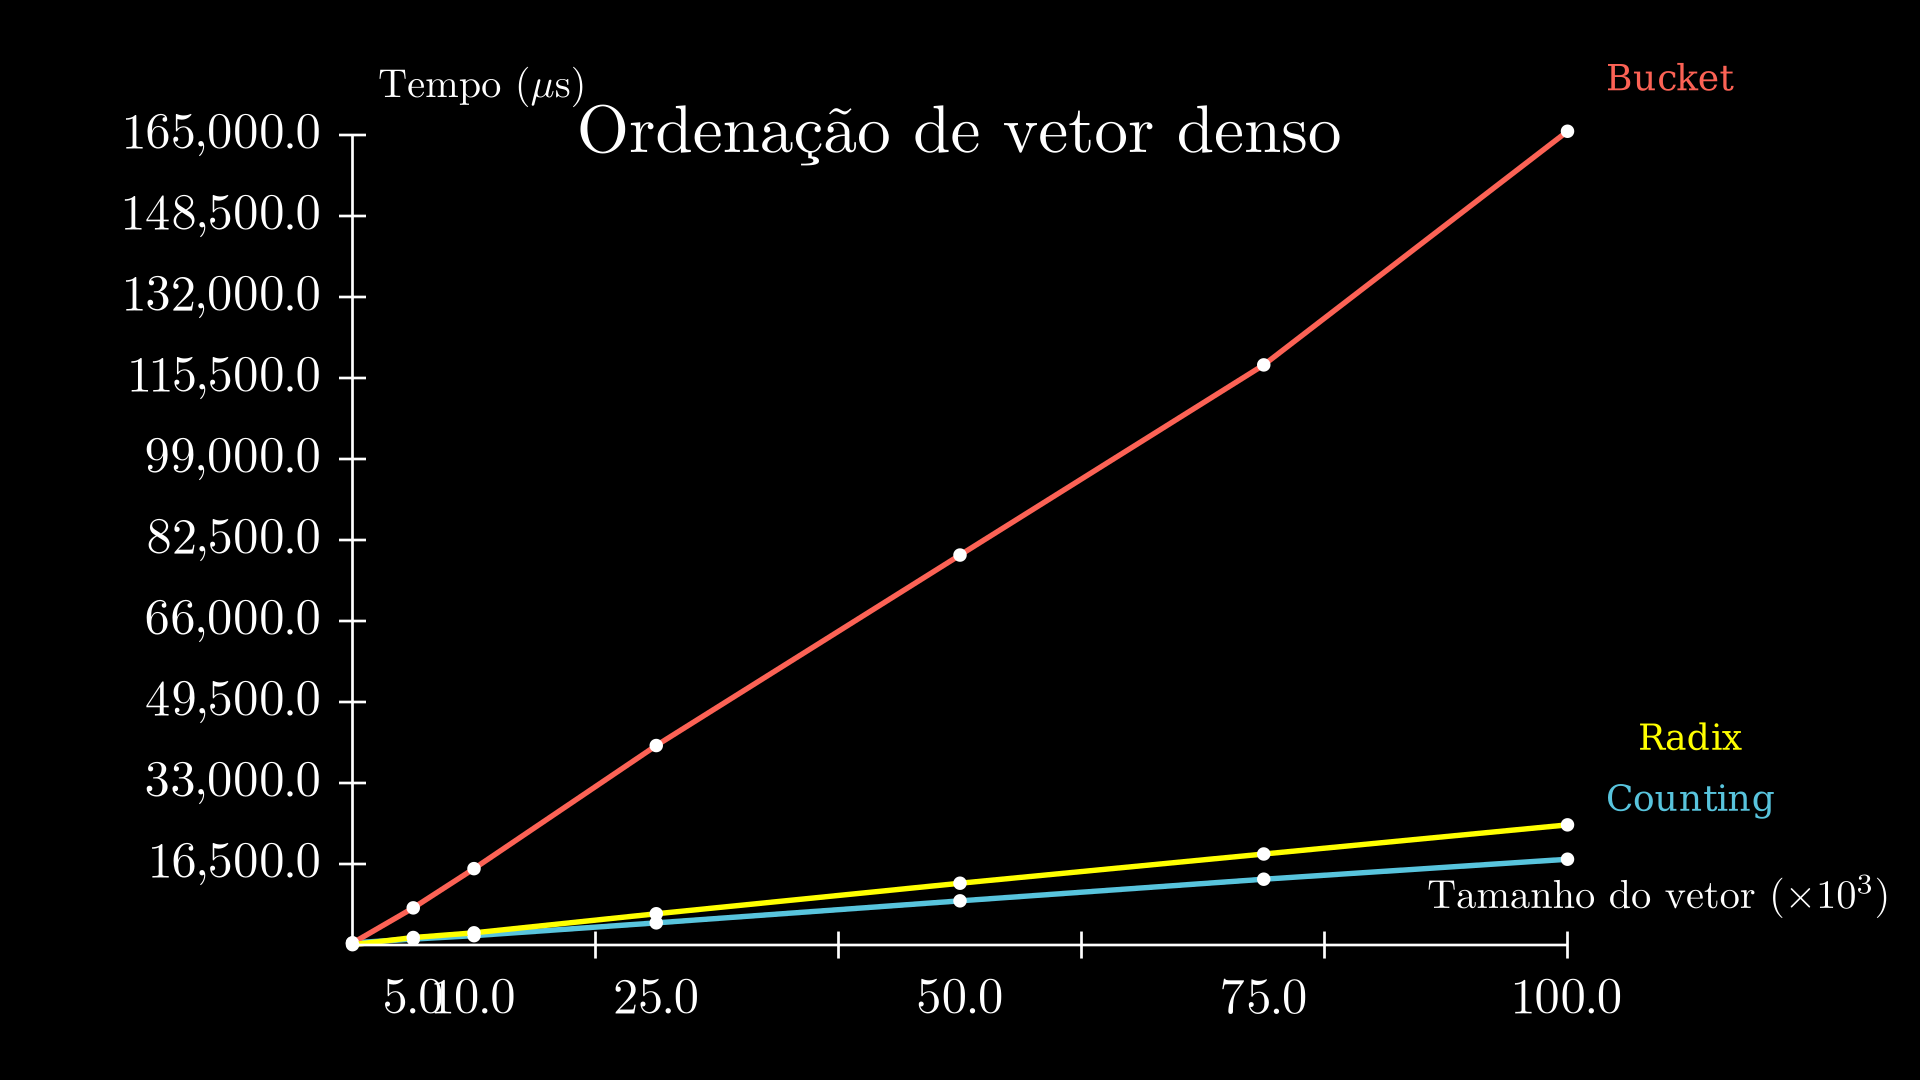
\includegraphics[width=\textwidth]{denso.png}
        \label{fig:denso}
      \end{figure}
      Ao comparar com o gráfico anterior (\ref{fig:uniforme}), é possível observar que isso realmente acontece. 
      O tempo médio passa de aproximadamente 32000 $\mu s$ s para 16000 $\mu s$. 
    \newpage
    \subsection{Vetor Esparso}
      Ao contrário do denso, o vetor esparso possui os elementos espalhados e pouca repetição.
      O valor máximo é até $100\times$ o tamanho do vetor. Logo, a complexidade é 
      $O(n+k) \rightarrow O(n+100n)$, isto é, $55.5\times$ pior que no vetor uniforme para Counting e 
      Bucket \ref{fig:uniforme}. Entretanto, com a escolha correta de base para o Radix, é possível manter baixo tempo de
      execução, como mostrado em \ref{fig:esparso}.
      \begin{figure}[H]
        \caption{Ordenação de vetores esparsos com até 100000 elementos}
        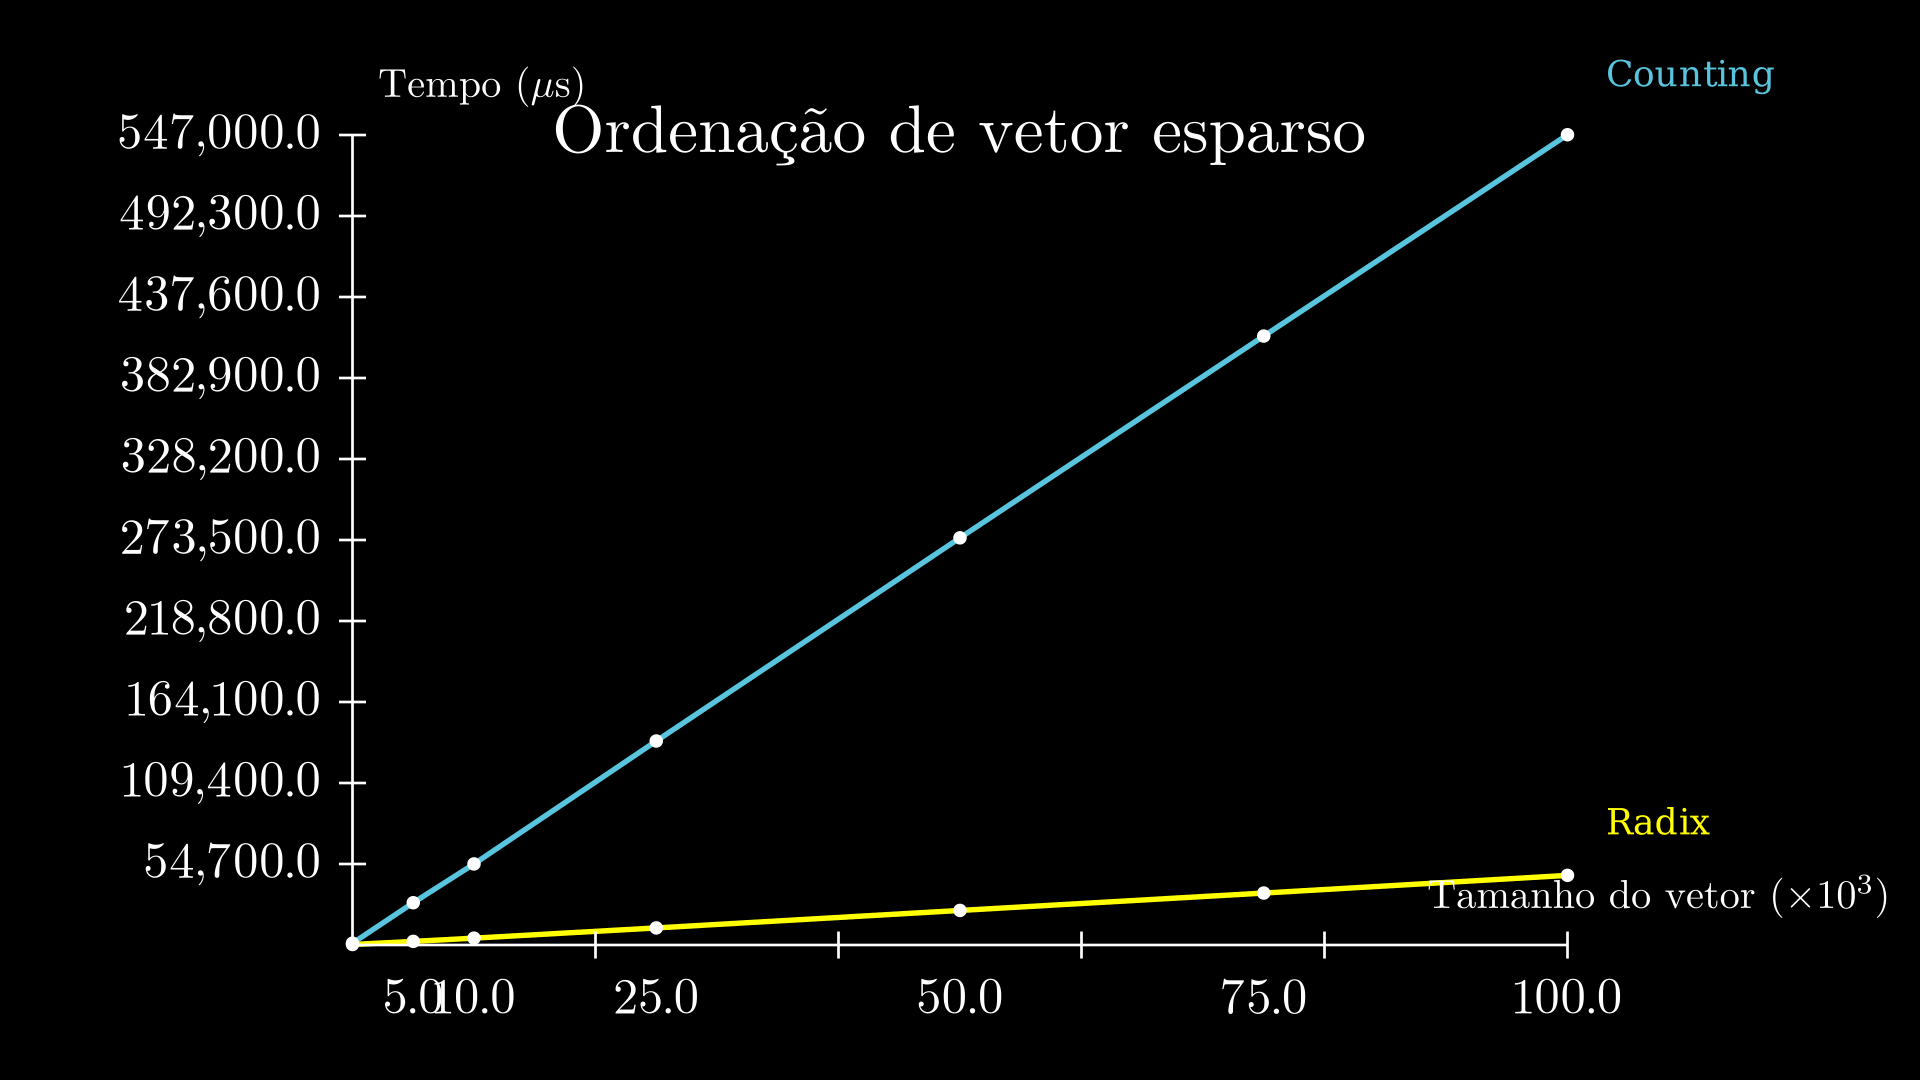
\includegraphics[width=\textwidth]{esparso1.png}
        \label{fig:esparso}
      \end{figure}
      O computador não conseguiu suportar o alto custo de espaço do Bucket Sort, com milhares de listas
      encadeadas, excedendo a memória reservada para o funcionamento do algoritmo e assim sendo retirado
      do gráfico. 
      \\ Nos algoritmos restantes, entretanto, Counting funciona muito mal, devido ao alto valor de $k$, 
      enquanto com um bom $b$, o Radix continua com pequena constante.
    \newpage
    \subsection{Base do Radix}
      O diferencial dos dois outros métodos para o Radix Sort é a escolha de base, que permite ao 
      algoritmo quebrar um número em partes para ordenar com tempo linear e baixo tempo de 
      execução em qualquer situação. O gráfico \ref{fig:radixBase} mostra porque a melhor escolha de base é
      $b=n$.
      \begin{figure}[H]
        \caption{Eficiência de algumas bases comuns no Radix Sort ordenando vetores esparsos}
        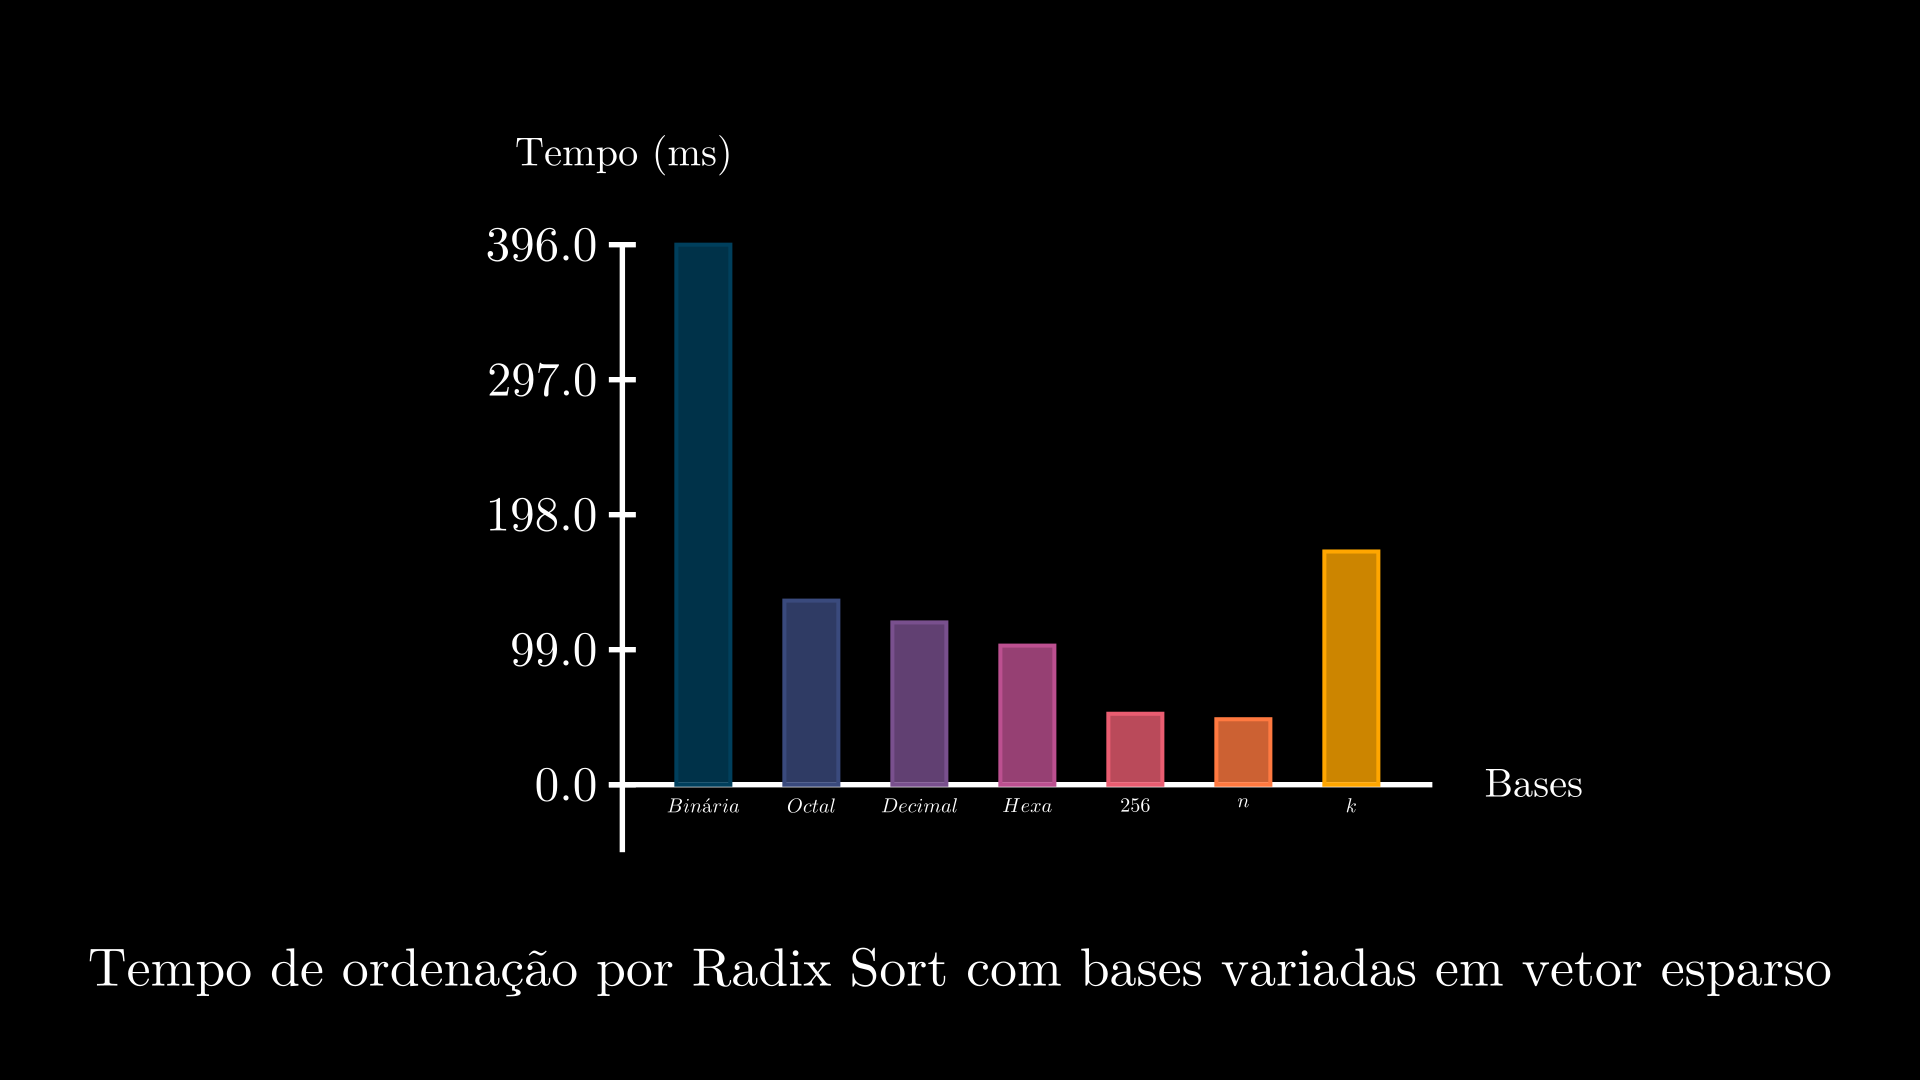
\includegraphics[width=\textwidth]{bargraph.png}
        \label{fig:radixBase}
      \end{figure}
      Nesse gráfico foi utilizado um vetor de tamanho 100000 e máximo de 10000000. 
      De todos as bases, binária, decimal, octal, $k$, a que melhor performa é $n$.
      Assim, confirmam-se os cálculos feitos na parte de metodologia sobre o Radix Sort. \ref{radix}
      apesar de ainda linear, é bem pior que o Radix. 
    \subsection{Comparação com outros métodos}
      Também é preciso comparar os métodos estudados nesse relatório com os passados. Ainda que 
      os lineares tendam a ser melhores no geral, cada um tem suas nuances e especializações, de forma
      que é importante analisar a situação antes de escolher o método com o qual se deseja trabalhar.
      Para a construção do gráfico \ref{fig:met1} foram utilizados vetores de tamanho 10000 a 50000, randomicamente 
      gerados.
      % \\[\baselineskip] 
      \begin{figure}[H]
        \caption{Os métodos de ordenação estudados ao longo do semestre}
        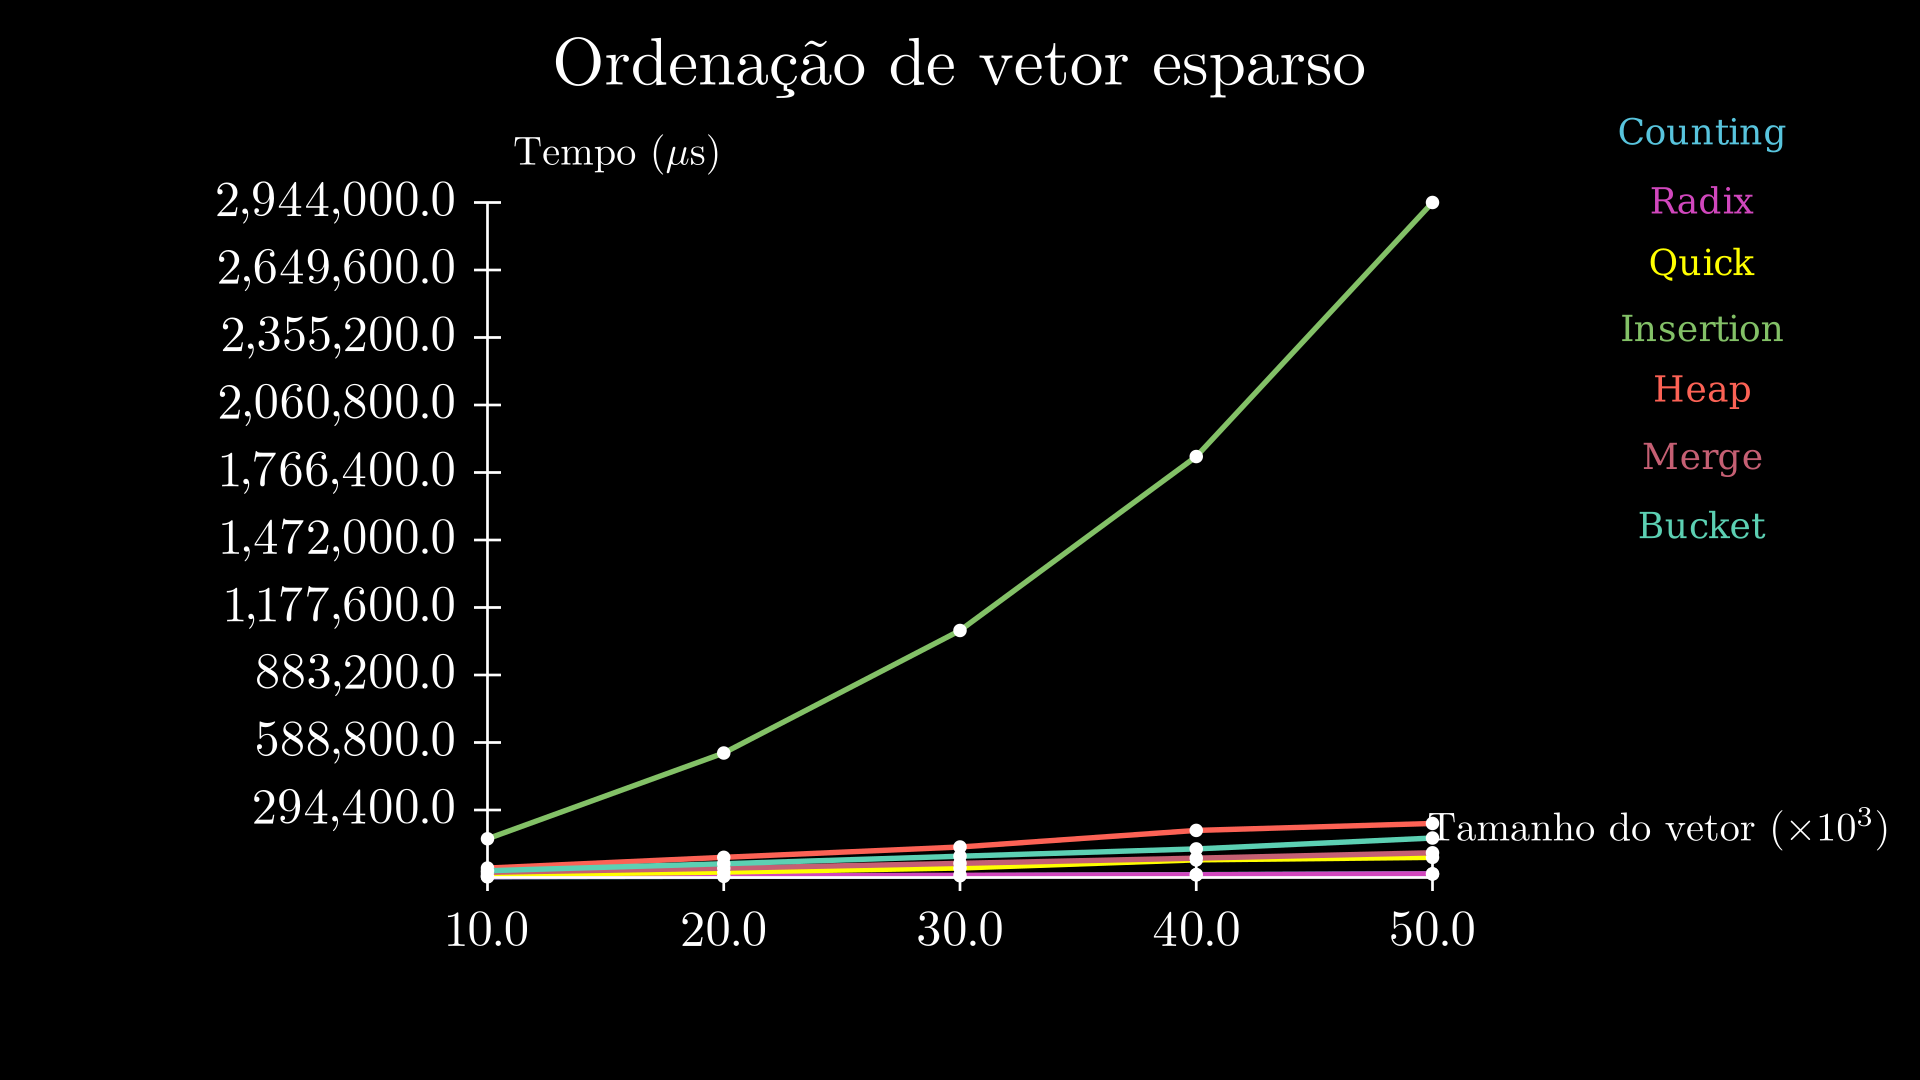
\includegraphics[width=\textwidth]{allmethods1.png}
        \label{fig:met1}
      \end{figure}
      \begin{figure}[H]
        \caption{Exclui-se o método com eficiência quadrática para permitir melhor visualização}
        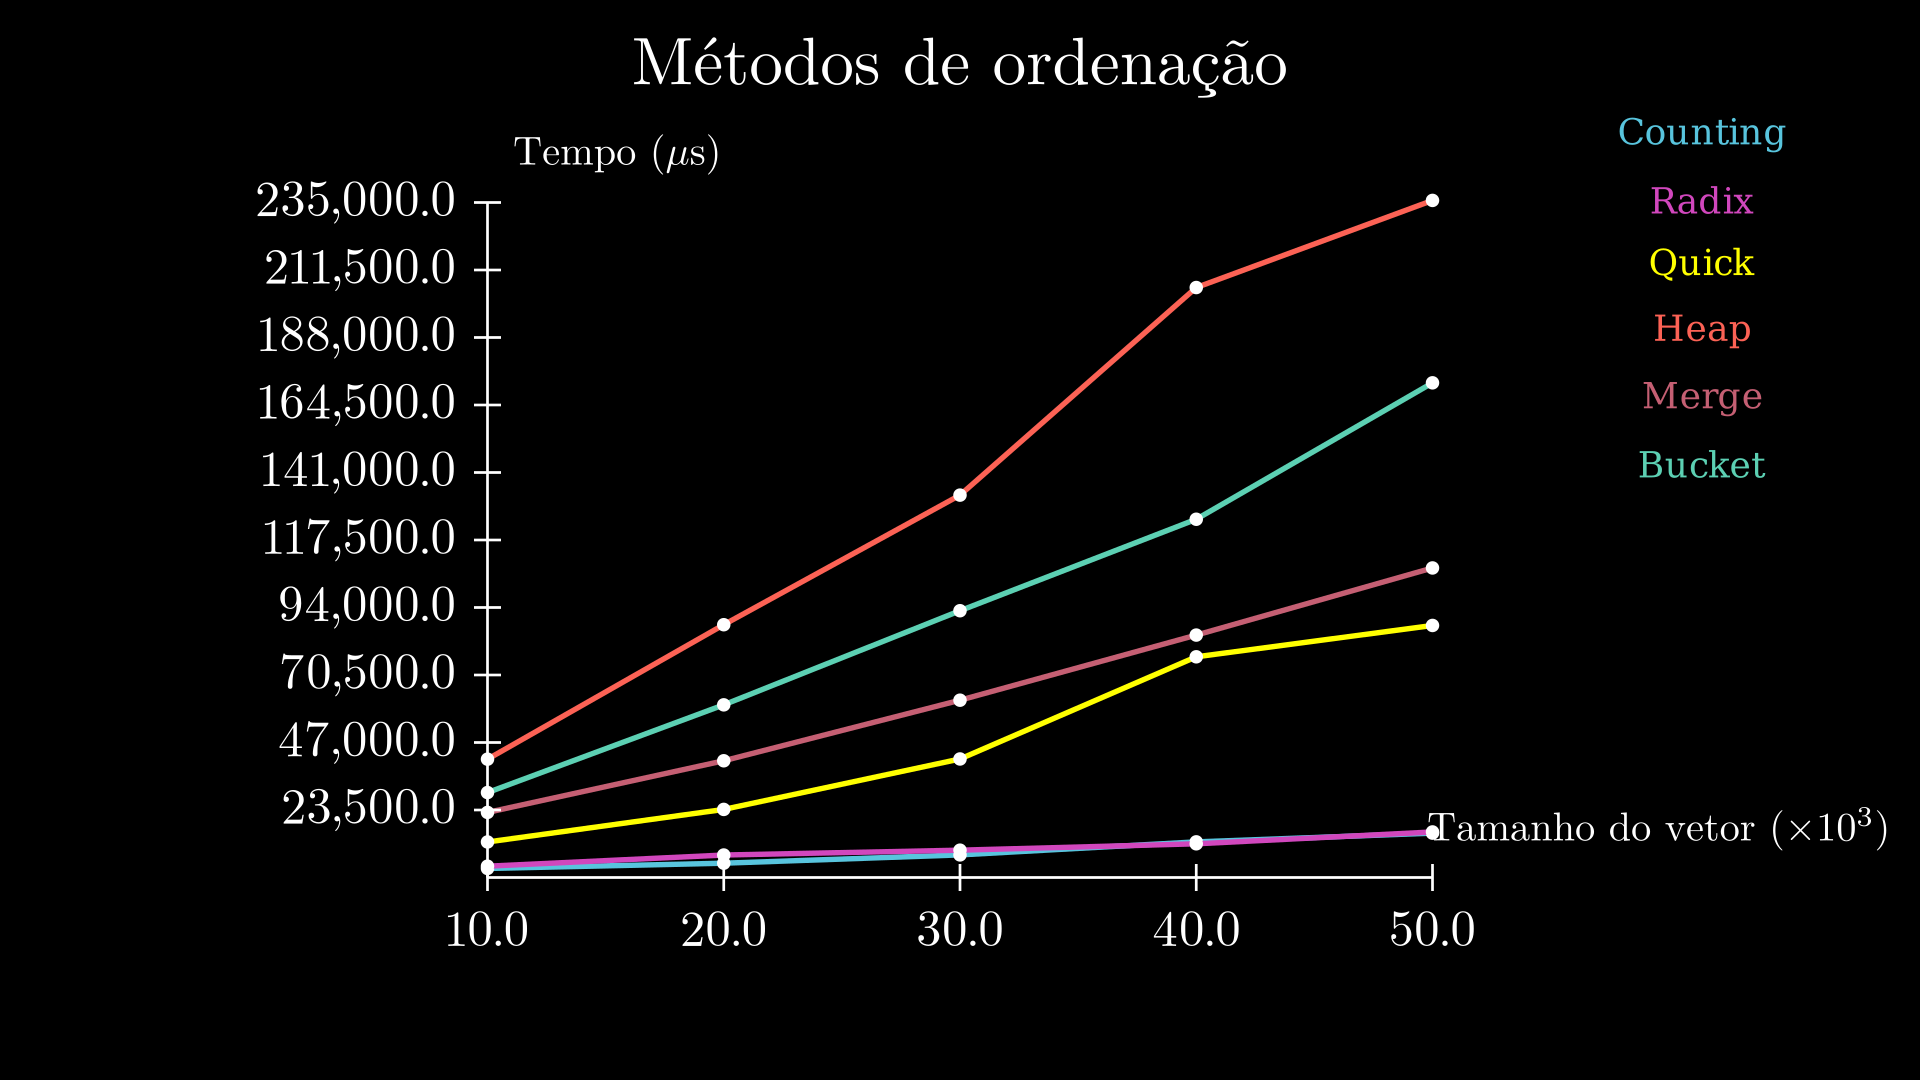
\includegraphics[width=\textwidth]{allmethods2.png}
        \label{fig:met2}
      \end{figure}
      O Insertion, de complexidade $O(n^2)$, atrapalha a análise dos outros métodos.
      Ao retirá-lo, obtemos o gráfico \ref{fig:met2}, no qual é possível observar os 
      métodos de contagem se sobressaindo, enquanto 
      aqueles que utilizam comparação se mostram mais demorados.

\section{Conclusão}
    %%%%%% Conclusão do relatório. O que você aprendeu nessa tarefa? %%%%%%
    Durante a elaboração desse relatório, além de aprender mais sobre a ferramenta LaTeX,
    foi possível constatar a eficiência dos métodos estudados na teoria, bem como comparar com o que havia
    sido estudado ao longo do ano. Com o Bucket Sort sofrendo por \textit{Stack Overflow}, foi possível 
    entender quão grave é a super utilização de ponteiros. Também pude constatar que a utilização da base $n=k$ é a 
    mais eficiente dentre todas, no método mais eficiente. Por fim, da comparação com outros métodos que estudamos
    ao longo do ano, foi possível comparar a linearidade e linear-logaritmicidade entre eles.
\printbibliography[heading=bibintoc, title={Referências}]
    %%%%%% Lembre-se de adicionar as referências bibliográficas utilizadas no arquivo 'references.bib'e depois cita-las nessa seção. Conulta: https://pt.overleaf.com/learn/latex/Bibliography_management_in_LaTeX %%%%%%

\end{document}

 